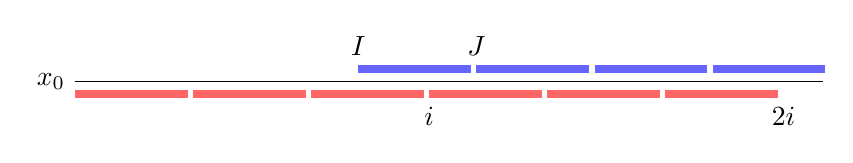
\begin{tikzpicture}
\draw[-] (0,0) -- (9.5,0);
\foreach \x in {0,1.5,...,7.6}{
\fill[red!60] (\x,-3pt) rectangle +(1.43,-3pt);
}
\node (I) at (3.6,0.2) [above] {$I$};
\node (J) at (5.1,0.2) [above] {$J$};
\foreach \x in {3,4.5,...,7.5}{
\fill[blue!60] (\x+0.6,3pt) rectangle +(1.43,3pt);
}
\node (i) at (4.5,-0.2) [below] {$i$};
\node (2i) at (9,-0.2) [below] {$2i$};
\node (x0) at (-0,0) [left] {$x_0$};
\end{tikzpicture}